\begin{frame}{What is a hyperplane?}
\begin{columns}
  \begin{column}{0.55\textwidth}
    \begin{itemize}
      \item In $p$-dimensional space, a hyperplane is a $(p-1)$-dimensional affine subspace.
      \item In 2D, a hyperplane is a flat 1D subspace, aka a line.
      \item In 3D, a hyperplane is a flat 2D subspace, aka a plane.
    \end{itemize}
  \end{column}
  \begin{column}{0.45\textwidth}
    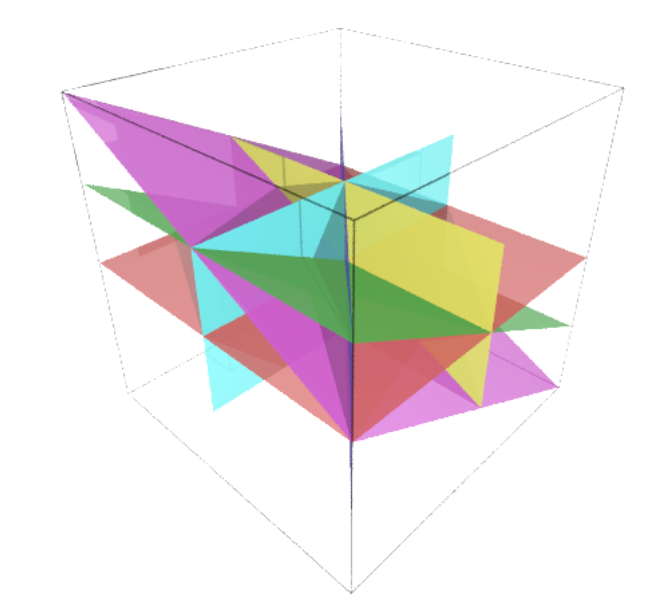
\includegraphics[width=\textwidth]{images/support-vector-machines/support-vector-machines-2.png}
  \end{column}
\end{columns}
\end{frame}


\begin{frame}{Mathematical Definition}
\begin{itemize}
  \item A 2D hyperplane is defined by the equation:
  \[
  \beta_0 + \beta_1 X_1 + \beta_2 X_2 = 0
  \]
  \item “Define” means any $\mathbf{X} = (X_1, X_2)$ for which the above equation holds is a point on the hyperplane.
  \item The above equation describes a line, which is a hyperplane in 2D.
\end{itemize}
\end{frame}


\begin{frame}{Mathematical Definition}
\begin{itemize}
  \item In \( p \) dimensions, a hyperplane is defined by the equation:
  \[
  \beta_0 + \beta_1 X_1 + \dots + \beta_p X_p = 0
  \]
  \item Similarly, any \( \mathbf{X} = (X_1, X_2, \dots, X_p) \) for which the above equation holds is a point on the hyperplane.
\end{itemize}
\end{frame}


\begin{frame}{Separating Hyperplane}
\begin{itemize}
  \item Instead of a point on the hyperplane, consider \( \mathbf{X} \) for which
  \[
  \beta_0 + \beta_1 X_1 + \dots + \beta_p X_p > 0
  \]
  \item This point lies on one side of the hyperplane. An \( \mathbf{X} \) for which
  \[
  \beta_0 + \beta_1 X_1 + \dots + \beta_p X_p < 0
  \]
  lies on the other side of the hyperplane.
  \item We can think of the hyperplane as dividing the \( p \)-dimensional space into two halves.
\end{itemize}
\end{frame}

\begin{frame}{Separating Hyperplane}
\begin{columns}
  \begin{column}{0.5\textwidth}
    \centering
    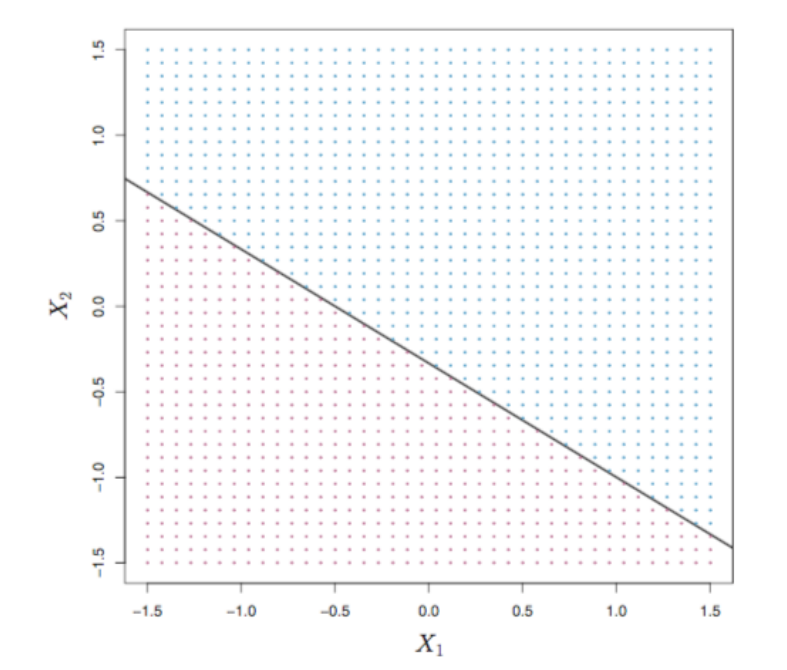
\includegraphics[width=\linewidth]{images/support-vector-machines/support-vector-machines-3.png}
    
    {\scriptsize\textit{ISL (8th printing, 2017)}}
  \end{column}
  \begin{column}{0.48\textwidth}
    \begin{itemize}
      \item This hyperplane in 2 dimensions is the line
      \[
        1 + 2X_1 + 3X_2 = 0
      \]
      \item The blue region is the set of points for which
      \[
        1 + 2X_1 + 3X_2 > 0
      \]
      \item The purple region is the set of points for which
      \[
        1 + 2X_1 + 3X_2 < 0
      \]
    \end{itemize}
  \end{column}
\end{columns}
\end{frame}


\begin{frame}{Separating Hyperplane Classifier}
\begin{columns}
  \begin{column}{0.55\textwidth}
    \begin{itemize}
      \item \textbf{Idea:} Use a separating hyperplane for binary classification.
      \item \textbf{Key assumption:} Classes can be separated by a linear decision boundary.
    \end{itemize}
  \end{column}
  \begin{column}{0.45\textwidth}
    \centering
    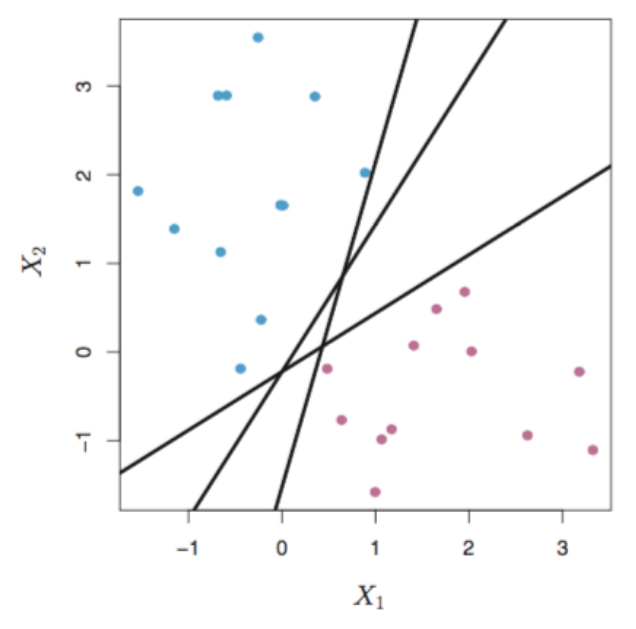
\includegraphics[width=\linewidth]{images/support-vector-machines/support-vector-machines-4.png}

    {\scriptsize\textit{ISL (8th printing, 2017)}}
  \end{column}
\end{columns}
\end{frame}

\begin{frame}{Separating Hyperplane Classifier}
\begin{itemize}
  \item \textbf{Aside:} Logistic regression effectively finds a separating hyperplane.
\end{itemize}

\centering
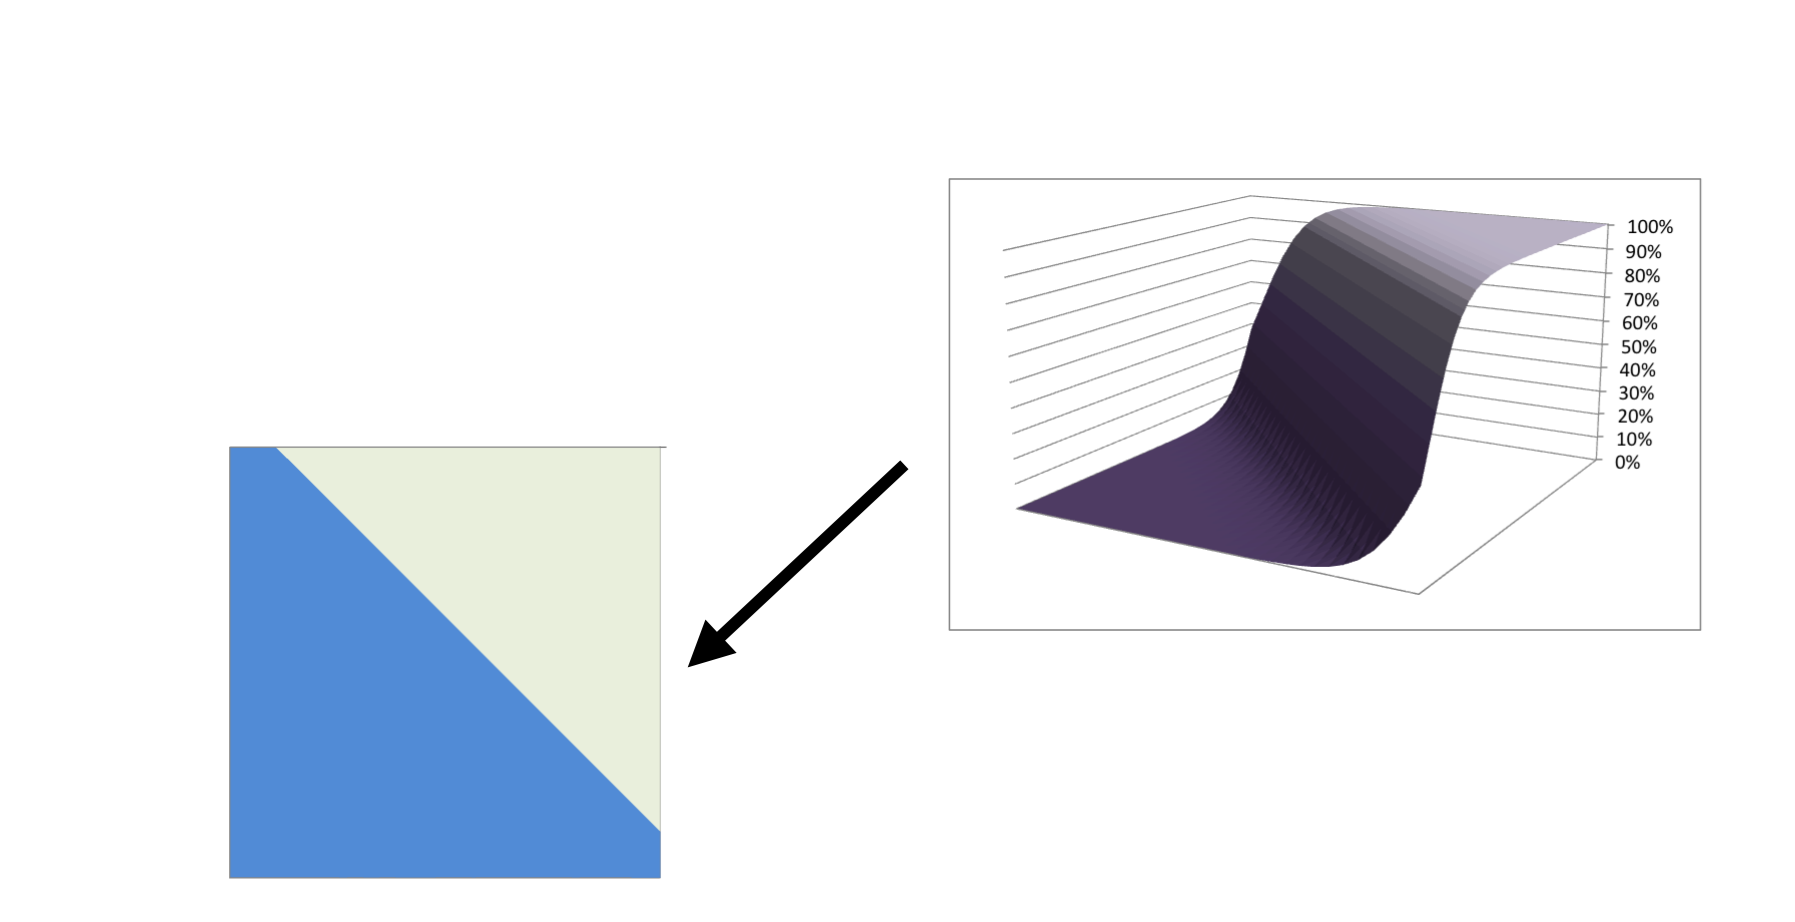
\includegraphics[width=0.75\linewidth]{images/support-vector-machines/support-vector-machines-5.png}

\vspace{1em}

\begin{itemize}
  \item Maximal margin classifiers and SVMs do this differently.
\end{itemize}
\end{frame}


\begin{frame}{Separating Hyperplane Classifier}
\begin{columns}
  \begin{column}{0.5\textwidth}
    \begin{itemize}
      \item \textbf{To classify new data points:}
      \item Assign class by location of new data point with respect to the hyperplane.
    \end{itemize}

    \[
      \hat{y} = \text{sign}(\beta_0 + \beta_1 x_1 + \ldots + \beta_p x_p)
    \]

    \begin{itemize}
      \item The farther away a point is from the separating hyperplane, the more confident we are about its class assignment.
    \end{itemize}
  \end{column}

  \begin{column}{0.5\textwidth}
    \centering
    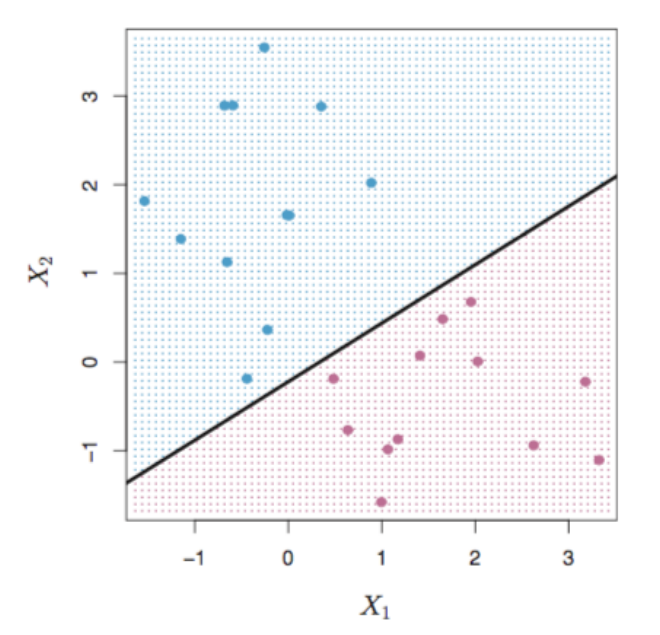
\includegraphics[width=\linewidth]{images/support-vector-machines/support-vector-machines-6.png}
  \end{column}
\end{columns}
\end{frame}


\begin{frame}{Separating Hyperplane Classifier}
\begin{columns}
  \begin{column}{0.55\textwidth}
    \begin{itemize}
      \item Notice that for a linearly separable dataset, there are many possible separating hyperplanes that divide the dataset into two classes (in fact, an infinite number).
    \end{itemize}
  \end{column}
  \begin{column}{0.45\textwidth}
    \centering
    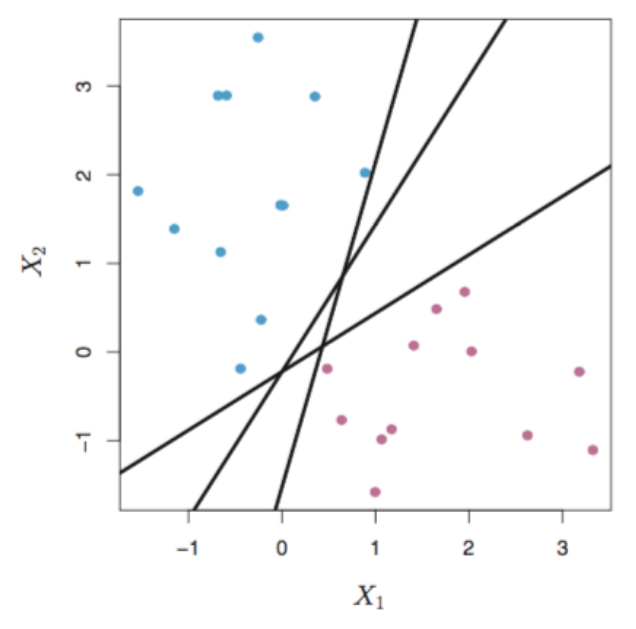
\includegraphics[width=\linewidth]{images/support-vector-machines/support-vector-machines-4.png}
  \end{column}
\end{columns}
\end{frame}
